\chapter{Small oscillations}
\section{Potential energy and equilibrium}
In order to understand the general theory of oscillations, it is essential to know about the potential energl at the equilibrium configuration. Let us consider a conservative system in which the potential energy is: function of position only. Let the system be specified by $n$ generalized coordinates $q_{1}, q_{2}, \ldots, q_{n}$, not involve, time explicitly. For such a system, the potential energy is given by
$$
V=V\left(q_{1}, q_{2}, \ldots, q_{n}\right)
$$
and the generalized forces are given by
$G_{k}=-\frac{\partial V}{\partial q_{k}}$ where $k=1,2, \ldots ., n$\\
The system is said to be in equilibrium, if the generalized forces acting on the system are equal to zero: i.e.,
$$
G_{k}=-\left[\frac{\partial V}{\partial q_{k}}\right]_{0}=0
$$
\subsection{Stable,Unstable and Neutral equilibrium}
\subsubsection{Stable equilibrium}
A system is said to be in stable equilibrium, if a small displacement of the system from the rest position (by giving a little energy to it) results in a small bounded motion about the equilibrium position.
\subsubsection{Unstable equilibrium}
Small displacement of the system from the equilibrium position results in an unbounded motion, it is in an unstable equilibrium.
\subsubsection{Neutral equilibrium}
 Further, if the system on displacement has no tendency to move about or away the equilibrium position, it is said to be in neutral equilibrium.\\
 \begin{minipage}{0.5\textwidth}
 \begin{figure}[H]
 	\centering
 	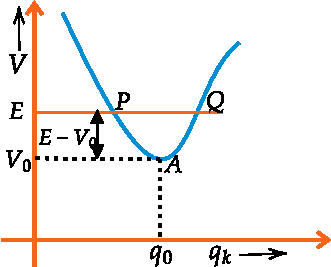
\includegraphics[height=4cm,width=5cm]{stable}
 	\caption{}
 	\label{}
 \end{figure}
 \end{minipage}
\begin{minipage}{0.5\textwidth}
\begin{figure}[H]
	\centering
	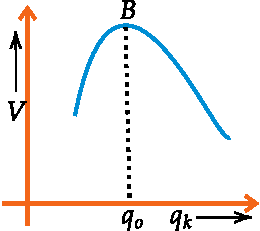
\includegraphics[height=3cm,width=5cm]{unstable}
	\caption{}
	\label{}
\end{figure}
\end{minipage}
A graph drawn between the potential energy of the system and a particular coordinate $q_{k}$ is called potential energy curve and  The positions $A$ and $B$, where the generalized force $F=-\partial V / \partial q$ vanishes, are the positions of equilibrium; potential energy $V$ is minimum (say $V_{0}$ ) at $A$ [Fig 4.1] and maximum at $B$ [Fig 4.2 ]. Position $A$ corresponds to the stable equilibrium, because if the system is displaced from $A$ to $Q$ by giving energy $\left(E-V_{0}\right)$ and left to itself, the system tries to come in the position of minimum potential energy. Consequently the potential energy will change to kinetic energy and at $A$ the energy $\left(E-V_{0}\right)$ will be purely in the kinetic form because of the conservation law. This will change again to potential form, when the system moves towards the position $P$ and hence a bounded motion ensues about the equilibrium position $A$. Obviously the position $B$ of the maximum potential energy represents the unstable equilibrium because any energy given to the system at this position will result more and more kinetic energy when the system moves either left or right to it. In this case, the system moves away from the equilibrium position. In case of neutral equilibrium, the potential energy is independent of the coordinate and equilibrium. occurs at any arbitrary value of that coordinate.
\section{Small oscillations}
In small oscillation we generalize the harmonic oscillator problem of one degree of freedom in the lagrangian formulation to the case of small amplitude oscillations of a system of seversl degrees of freedom near the position of equilibrium.When we go from a single oscillator to the problem of two coupled oscillators the analysis results in some interesting and surprising new features.We shall see that the motion of the two coupled oscillators in general is much complicated and none of the oscillators in general executes simple harmonic motion.However for small amplitude oscillations ,we may express the general motion as a superposition of two independant simple harmonic motions ,both going on simultaneously.We call thsese two simple harmonic motions as normal modes or simply modes.Further we shall see that a system of N coupled oscillators with N degrees of freedom ,has exactly N independant modes of vibration and general motion can be expressed as the superposition of N normal modes.Each mode has its own frquency and wavelength.
\subsection{Matrix method to solve small oscillations}
\begin{figure}[H]
	\centering
	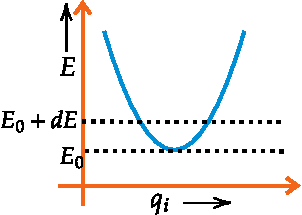
\includegraphics[height=3cm,width=5cm]{potential}
	\caption{}
	\label{}
\end{figure}